\section{Fixed workflows}
\label{sec:fixed}

\begin{upshot}
\item \textbf{A fixed workflow is defined by who decides, and when.} We settle every control
  decision at design time: which operation runs next, how many model calls the run makes, and
  what ends it. The model is called at points we choose, and what it returns is content that
  travels through the graph without changing the graph.
\item \textbf{The fixed shape is what we buy.} One shape per run means the cost is known before
  the run starts, a failure belongs to the stage that produced it, and the run ends because the
  graph ends rather than because a counter ran out.
\item \textbf{The fixed shape is also what we pay.} Our environment is partially observable, so
  the evidence a decision needs may not exist until an action produces it. A graph with no edge
  back has nowhere to ask a second question, and the question it cannot ask is the one its own
  output depended on.
\item \textbf{The sections that follow give these decisions away one at a time.} \Cref{sec:reactive}
  hands the choice of the next action to the model, \cref{sec:planning} puts the intended sequence
  into state where it can be revised and moves acceptance off the component that proposed the work,
  and \cref{sec:reflection} lets one attempt change the context of the next. Every move costs
  something the fixed shape was giving us for free, so every move has to be earned.
\end{upshot}

\subsection{Control decisions and content decisions}
\label{sec:fixed-decisions}

\begin{definition}[Fixed workflow]
\label{def:fixed-workflow}
A \emph{fixed workflow} is an agent program in which we make every control decision at design time. The operations, the order they run in, the number of model calls, and the condition that ends the run are all written before the program sees a task. The model supplies content at points we choose. Such a program sits at one end of an axis the definition of rationality already gave us: ``To the extent that an agent relies on the prior knowledge of its designer rather than on its own percepts and learning processes, we say that the agent lacks autonomy'' \citep[\S2.2.3]{russell2020aima}.
\end{definition}

Two kinds of decision run through any agent program: i) control decisions and ii) content
decisions. 

A \emph{control decision} selects what the program does next: which operation runs,
whether anything runs after it, and when the program stops. A \emph{content decision} fills in a
value that an operation needs: which file looks suspicious, what a patch says, which lines are
worth reading. 

The distinction is not about difficulty. What I mean is, naming the file to patch is the harder
problem (and the model decides that for us). Deciding that a file is named before lines are read is the one that fixes the shape of
the run (and that's something that we do). \Cref{tab:fixed-decisions} sorts the decisions of an agent program on that line.

\begin{table}[htbp]
  \caption{The decisions an agent program makes, and where a fixed workflow puts each one.}
  \label{tab:fixed-decisions}
  \small
  \begin{tabularx}{\linewidth}{Xlll}
    \toprule
    Decision & Kind & Who decides & When \\
    \midrule
    Which operation runs next & Control & We do & Design time \\
    Whether another operation runs after this one & Control & We do & Design time \\
    How many model calls the run makes & Control & We do & Design time \\
    What ends the run & Control & We do & Design time \\
    Which artifacts a step reads and writes & Control & We do & Design time \\
    \midrule
    What a model call returns & Content & The model & Run time \\
    Which values travel to the next step & Content & The model, within our schema & Run time \\
    \bottomrule
  \end{tabularx}
\end{table}

Fixed does not mean straight. A fixed workflow may branch, filter, and repeat a step a set
number of times; what makes it fixed is that we wrote the predicate on which it branches, so the
set of paths through the program is closed and we can enumerate it. The distinction that matters
is not one of graph topology but of authorship: \textbf{in a fixed workflow no model output is ever read
as an instruction about what to do next. It is read as data}.

\subsection{What we gain and what we lose}
\label{sec:fixed-tradeoff}

Fixed workflows can be a double-edged sword. They give us predictability and control, but at the cost of flexibility and adaptability.

\subsubsection{What we gain}
Three guarantees come with fixing the control decisions: i) the run has one shape, ii) a failure
has an address, and iii) the run terminates by construction. 
\bi

\item \textbf{Shape.} The run has one shape, so its cost is countable before it starts. The model calls are the ones we wrote, and their number does not depend on what the model says. We can put a token budget on a task
before we have read the task.

\item \textbf{Failure mode.} A failure has an address. Every intermediate artifact is produced by a named step, so a wrong
answer belongs to the step that produced it, and debugging a bad patch means reading four
artifacts rather than reconstructing a forty-turn trajectory.

\item \textbf{Termination.} The run terminates because the last operation returns. That is a fact about the program text and
not a claim about the model's behavior (and it is the one guarantee the later versions never get
back: they replace it with a model-call budget, which guarantees stopping but says nothing about
finishing).

\ei

Our prior knowledge is doing all of this work, and doing it legitimately: ``As a practical matter,
one seldom requires complete autonomy from the start: when the agent has had little or no
experience, it would have to act randomly unless the designer gave some assistance''
\citep[\S2.2.3]{russell2020aima}. A fixed workflow is the limiting case of that assistance, where
the designer supplies the whole program and leaves for the model only the words.

\subsubsection{What we lose}
The tradeoff is that a fixed workflow relies on assumptions we made when we designed it.
If new evidence shows that those assumptions were incomplete or wrong, it cannot change its
sequence of operations to investigate. This limits the autonomy a rational agent can have \citep[\S2.2.3]{russell2020aima}:
``A rational agent should be autonomous---it should learn what it can to compensate for partial or incorrect prior knowledge''.

What I mean is, it is rational exactly while our prior knowledge holds, and when that knowledge
turns out to be partial, the workflow does not notice. It has no representation of what it does
not know.

The shape of that failure is specific. Our environment is partially observable (\cref{sec:agents-environment}), 
so a rational agent here acts to see, and a fixed workflow does act to see \textit{but} it does its looking on a schedule we wrote before we knew 
what the looking would return. If the value the patch depends on comes from a helper the alert never named, no node exists in which to ask for it. 
The chain does not stall and it does not report a gap. It writes the patch anyway, because that's how we designed the workflow.

Now, all of this is not to say that a fixed workflow is useless; my point simply is that it has obvious limitations that stem from its reliance on prior knowledge.
In fact, \Cref{sec:fixed-agentless} discusses a concrete approach that actually demonstrates a successful realization of a fixed workflow. 
After that, the next few sections will explore more autonomous agents and see how they address the limitations of fixed workflows.

\subsection{Agentless, one realization}
\label{sec:fixed-agentless}

So far, our discussion has been about shape. Now let's see a system with that shape, and it is not a toy. 
Agentless resolves real GitHub issues by running three phases in a fixed order. It's a relatively older 
piece of work (October 2024) but it's worth looking at. Notably, it resolved more SWE-bench Lite issues 
than any open-source agent at that time, but at a fraction of their cost \citep[\S5.1]{xia2025agentless}.

\begin{figure}[htbp]
  \centering
  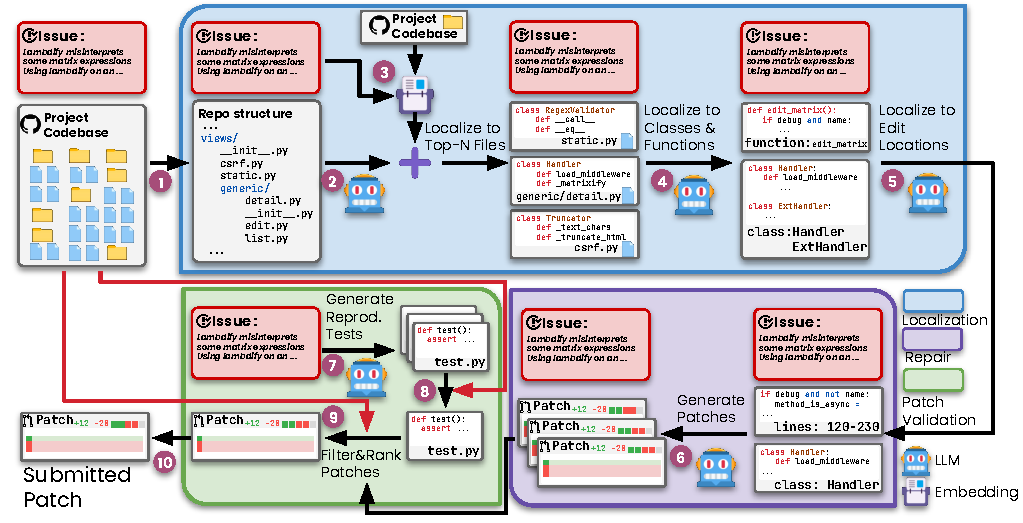
\includegraphics[width=\linewidth]{figures/agentless-fig1-overview.pdf}
  \caption{Agentless: localization (blue), repair (purple), and patch validation (green). The
  numbered steps are the whole program, and there is no arrow that a model output can redirect.
  Figure~1 of \citet{xia2025agentless}, reproduced from the authors' arXiv source (CC BY 4.0).}
  \label{fig:agentless-overview}
\end{figure}

The task is SWE-bench Lite: 300 problems, each one a real issue report and the Python repository
it was filed against, where the job is a patch that resolves the issue \citep{jimenez2024swebench}.
That is the job \msa{} does, on a different fixture.

Three phases, and the split from \cref{tab:fixed-decisions} is visible in every one of them. The
model fills in content; we fixed the order, the inputs, and the counts.

\bi

\item \textbf{Localization.} Three steps, each with a smaller input than the last. The repository
structure (directories and file names, no source text) yields the top three suspicious files; a
skeleton of those files (class and function headers, no bodies) yields the elements worth reading;
the full source of only those elements yields the edit locations \citep[\S3.1]{xia2025agentless}.
The model ranks and selects at every step, and it never asks for something the step did not hand
it (\cref{fig:seq-agentless}).

\item \textbf{Repair.} Each set of edit locations is widened by ten lines on either side, and the
model writes a patch in a search-and-replace format borrowed from Aider
\citep{gauthier2024aider}: the lines to find, and the lines to put in their place
(\cref{fig:search-replace}). Four location
sets, ten patches each, so forty candidates per issue \citep[\S3.2, \S4]{xia2025agentless}.

\item \textbf{Patch validation.} The model writes a test that reproduces the issue, and then the
runtime does the choosing. Candidates run against the repository's own passing tests, the
survivors run against the reproduction test, and the winner is the patch that occurs most often
once the survivors are normalized \citep[\S3.3]{xia2025agentless}.

\ei

\begin{figure}[htbp]
  \centering
  \resizebox{\linewidth}{!}{% One Agentless run. The pipeline initiates every call; the model only answers.
% Counts are the paper's defaults. Compare figures/seq-mini-swe-agent.tikz, where the
% controller initiates instead and the arrows therefore start on the other lifeline.
\begin{tikzpicture}[x=1cm, y=1cm,
  head/.style={gnode, minimum width=3.0cm, font=\sffamily\small},
  life/.style={draw=black!45, dashed},
  act/.style={-{Stealth[length=2.6mm]}, line width=1.4pt, draw=ibmblue},
  per/.style={-{Stealth[length=2.6mm]}, line width=1.4pt, draw=red!70!black},
  msg/.style={font=\sffamily\scriptsize, fill=white, inner sep=1.5pt, align=center},
  phase/.style={font=\sffamily\footnotesize\bfseries, fill=white, inner sep=2pt},
  note/.style={gnode, fill=black!6, font=\sffamily\scriptsize, align=center, inner sep=3pt}]

  \def\P{0} \def\M{7.4} \def\R{14.2}
  \node[head] (pipe) at (\P,0) {Pipeline (fixed)};
  \node[head] (mod)  at (\M,0) {Model};
  \node[head] (repo) at (\R,0) {Repository and tests};
  \draw[life] (pipe.south) -- (\P,-12.5);
  \draw[life] (mod.south)  -- (\M,-12.5);
  \draw[life] (repo.south) -- (\R,-12.5);

  \draw[black!25] (-1.1,-0.75) -- (15.3,-0.75);
  \node[phase] at (7.1,-0.75) {Localization};
  \draw[act] (\P,-1.45) -- (\M,-1.45) node[msg, midway, above] {structure format and the issue:\\which three files are suspicious?};
  \draw[per] (\M,-2.2) -- (\P,-2.2) node[msg, midway, above] {three file names};
  \draw[act] (\P,-2.9) -- (\R,-2.9) node[msg, midway, above] {embed the files that survive folder filtering, retrieve by similarity to the issue};
  \draw[act] (\P,-3.6) -- (\M,-3.6) node[msg, midway, above] {skeletons of those files:\\which classes and functions?};
  \draw[per] (\M,-4.35) -- (\P,-4.35) node[msg, midway, above] {the elements worth reading};
  \draw[act] (\P,-5.05) -- (\M,-5.05) node[msg, midway, above] {their full source:\\which lines to edit? ($4$ samples)};
  \draw[per] (\M,-5.8) -- (\P,-5.8) node[msg, midway, above] {four sets of edit locations};

  \draw[black!25] (-1.1,-6.5) -- (15.3,-6.5);
  \node[phase] at (7.1,-6.5) {Repair};
  \draw[act] (\P,-7.2) -- (\M,-7.2) node[msg, midway, above] {context windows, $\pm 10$ lines:\\write a patch ($10$ per set)};
  \draw[per] (\M,-7.95) -- (\P,-7.95) node[msg, midway, above] {forty Search/Replace patches};

  \draw[black!25] (-1.1,-8.65) -- (15.3,-8.65);
  \node[phase] at (7.1,-8.65) {Patch validation};
  \draw[act] (\P,-9.35) -- (\M,-9.35) node[msg, midway, above] {write a test that reproduces the issue ($40$ samples)};
  \draw[per] (\M,-10.1) -- (\P,-10.1) node[msg, midway, above] {forty candidate tests};
  \draw[act] (\P,-10.8) -- (\R,-10.8) node[msg, midway, above] {apply each patch, run the regression suite, then run the reproduction test};
  \draw[per] (\R,-11.55) -- (\P,-11.55) node[msg, midway, above] {pass or fail, for every patch};
  \node[note, anchor=west] at (0.2,-12.2) {a majority vote over the survivors selects the patch to submit. The run ends};
\end{tikzpicture}
}
  \caption{One Agentless run, with the paper's default counts \citep[\S3, \S4]{xia2025agentless}.
  Blue arrows are calls the pipeline makes; red arrows are what comes back. Read it against
  \cref{fig:agents-sequence}, which uses the same colors for the same things: there every blue
  arrow leaves the agent, here not one of them leaves the model.}
  \label{fig:seq-agentless}
\end{figure}

\begin{figure}[htbp]
  \centering
  % Agentless's Search/Replace edit format (its Figure 3), redrawn on our own worked alert.
\begingroup
\lstset{basicstyle=\ttfamily\scriptsize, numberstyle=\tiny\color{ibmfg!55}, xleftmargin=2.6em,
        aboveskip=2pt, belowskip=2pt}

{\sffamily\footnotesize\bfseries Original file\quad\mdseries\demoref{testcode/BenchmarkTest00283.py}\par}
\begin{lstlisting}[numbers=left, firstnumber=46]
sql = f'SELECT username from USERS where password = \'{bar}\''
con = helpers.db_sqlite.get_connection()
cur = con.cursor()
cur.execute(sql)
\end{lstlisting}

{\centering\footnotesize $\downarrow$\enspace one model call returns the block below, and nothing else\par}

\begin{lstlisting}[numbers=none]
<<<<<<< SEARCH
sql = f'SELECT username from USERS where password = \'{bar}\''
=======
sql = 'SELECT username from USERS where password = ?'
>>>>>>> REPLACE

<<<<<<< SEARCH
cur.execute(sql)
=======
cur.execute(sql, (bar,))
>>>>>>> REPLACE
\end{lstlisting}

{\centering\footnotesize $\downarrow$\enspace the runtime matches each search block and substitutes its replacement\par}

{\sffamily\footnotesize\bfseries Edited file\par}
\begin{lstlisting}[numbers=left, firstnumber=46]
sql = 'SELECT username from USERS where password = ?'
con = helpers.db_sqlite.get_connection()
cur = con.cursor()
cur.execute(sql, (bar,))
\end{lstlisting}
\endgroup

  \caption{The Search/Replace edit format, on the worked alert of \cref{sec:fixed-agentless}. The model returns
  the middle block and never touches the file; the runtime matches each search block and
  substitutes its replacement. Small edits are cheaper than regenerating the region and leave less
  room for invention. Redrawn after Figure~3 of \citet{xia2025agentless}.}
  \label{fig:search-replace}
\end{figure}

In that third phase, acceptance is a test outcome and a vote, not a model's opinion of its own
work, so the thing that proposes a patch is not the thing that accepts one. \Cref{sec:validation} 
is about that separation, and the numbers say it pays: majority voting alone resolved 77 issues, 
adding the repository's regression tests took it to 81, and adding the generated reproduction test 
took it to 96 \citep[\S5.2.3]{xia2025agentless}.
Agentless resolved 96 of 300 problems (32.00\%) at an average of \$0.70 and 78,165 tokens per
issue. SWE-agent, running the same model, resolved 55 (18.33\%) at \$2.53 and 498,346 tokens
\citep[Table~1]{xia2025agentless}. That pair comes closest to isolating control structure: hold
the model fixed, change who decides what runs next, and the pipeline resolved more issues at about
a quarter of the cost and a sixth of the tokens. The two systems differ in more than their control
structure, so this is the strongest available comparison rather than a controlled experiment.


I'd take all of these results with a grain of salt. Two limitations qualify this comparison. 

\bi
  \item First, Agentless did not lead the full leaderboard:
several closed-source systems scored higher, including CodeStory Aide with 129 resolved issues
(43.00\%). Those systems released neither code nor execution trajectories, so we cannot examine
how their control structures contributed to their results \citep[Table~1]{xia2025agentless}.
  \item Second, SWE-bench Lite has problems as an evaluation set: 4.3\% of its issue descriptions include
the exact developer patch, 5.0\% suggest a solution the developers did not use, and 10.0\% lack
enough information to solve the issue \citep[\S6.1]{xia2025agentless}. The authors also report a
filtered subset of 249 problems that excludes these cases \citep[\S6.2]{xia2025agentless}.
\ei

The answer leakage in that second limitation motivates a precaution in our own fixture: we
exclude the answer key. OWASP BenchmarkPython stores expected results alongside its test cases
\citep{owasp-benchmarkpython}. If an agent can read those results, it can obtain the expected
answers without analyzing the code, so its score no longer cleanly measures the ability we want
to evaluate.

In a nutshell, on well-specified issues, a fixed workflow with an execution-based selector matched or
beat the agents of its day. What it does not show is that fixed workflows win in general. 
Our position in the course is narrower in that the design-time side of \cref{tab:fixed-decisions} 
is a serious engineering position that we will try to systematically remediate with structured autonomy.

The same shape over our own fixture would be shorter still, and it is worth seeing why. A scanner
alert already names the file and the line, so the two phases Agentless spends recovering them
collapse into a runtime lookup. What remains is a chain of four steps: read the flagged region, ask
the model which lines to change, ask it for the patch, and submit. Call that shape \emph{the
chain}. Its cost is two model calls and one read whatever the alert, its trace has the same four
entries every time, and it terminates because the last step returns.

What the chain cannot do is visible in that list before anything runs. \demoref{search} is one of
\msa{}'s four tools and no step in the chain can call it, so when the value a query interpolates
reaches the flagged line through a helper in another file, the chain patches what it was given. It
does not stall and it does not report a gap; it writes a plausible patch from the region it has,
and a check that the patch applies, touches the flagged line, and clears a rescan will still pass.
\Cref{sec:reactive} is where that limit is lifted.

HW1 uses both shapes, for the reasons this section gives. Its intake stage, which runs the scanners
and normalizes their alerts into one contract, is a fixed chain: known cost, named artifacts,
failures located by stage. Its investigation loop is not, because triage is where the second
question gets asked.

\subsection{Exercises}

\be

\item Agentless picks its final patch by a vote over test outcomes. Use
\cref{tab:fixed-decisions}. Say whether that is a control decision or a content decision, who
makes it, and when. What would have to change for the model to make it instead?

\item Count the model calls the chain makes per alert, before any run. Now name one cost of the
run that the count does not fix in advance.

\item A submission check that confirms the patch applies, touches the flagged line, and clears a
rescan will still accept a patch that deletes the query outright. Write a fourth check that rejects
it, then say why the chain cannot run your check with the tools it has.

\item Add a fifth step to the chain that calls \demoref{search} once on an identifier taken from
the flagged line. Which decision have you moved to run time, which have you kept at design time,
and what can still go wrong?

\ee

\subsection{Reading}

Before class: \citet{xia2025agentless}, \S1, \S\S3.1--3.2, and Figure~1. These notes also draw on
\S3.3 for patch validation, \S4 for the defaults, \S5.1 and Table~1 for the comparison, \S5.2.3
and Table~4 for the selection ablation, and \S\S6.1--6.2 for the benchmark analysis. Read the FSE
version (Proc.\ ACM Softw.\ Eng.\ 2, FSE, article FSE037). The arXiv preprint carries the
``Agentless'' title prefix and numbers its sections differently, so the section references above
will not find the right text in it.

\paragraph{Looking ahead.}
\Cref{sec:reactive} moves the first row of \cref{tab:fixed-decisions} to run time: the model
chooses which operation runs next, and the graph grows an edge back. That is what a partially
observable environment asks for, since acting is how the agent sees, and it is what buys the
second question the chain cannot ask. It also spends all three guarantees we counted in
\cref{sec:fixed-tradeoff}. The cost of a run stops being countable in advance, a failure stops
having a single address, and termination stops being a fact about the program text, so the loop arrives
carrying a model-call budget, a terminal status, and a trace.
